\documentclass[a4paper,fleqn]{cas-dc}

%% ---- Citations: author-year style, e.g. (Sung et al., 2021) ----
\usepackage[authoryear]{natbib}

%% ---- Multi-panel figures: \begin{subfigure}... (Fig. 1a, 1b) ----
\usepackage{subcaption}

%% IMPORTANT: do NOT load graphicx, amsmath, amsfonts, amssymb, booktabs,
%% multirow, makecell, array, colortbl, dcolumn, hyperref or xcolor here.
%% cas-dc.cls already loads all of them; re-loading triggers option clashes.

%% ---- Optional extras (uncomment only if you need them) ----
%\usepackage{threeparttable}   % footnotes/notes inside tables
%\usepackage{siunitx}          % decimal-aligned numbers & units in tables
%\usepackage{orcidlink}        % \orcidlink{0000-0000-0000-0000}

%% ---- Author convenience macros (optional) ----
% \newcommand{\gene}[1]{\textit{#1}}   % italicise gene names, e.g. \gene{FHL1}

\begin{document}
\let\WriteBookmarks\relax
\def\floatpagepagefraction{1}
\def\textpagefraction{.001}

%% ===================== FRONT MATTER =====================
\shorttitle{A Compact 5-Gene Signature for Breast Cancer}
\shortauthors{H. Akmal and N. Kumar}
\title[mode=title]{A Compact 5-Gene Signature (FHL1, PCK1, ACVR1C, FABP4, and MT1H) for Diagnostic Prediction and Immune Characterization in Breast Cancer: An Integrated Machine Learning Approach}

\author[1]{Huzaifa Akmal}
\affiliation[1]{organization={Sanata Dharma University},
            city={Yogyakarta},
            country={Indonesia}}

\author[2]{Narendar Kumar}
\cormark[1]
\ead{narendar.kumar@utbm.fr}
\affiliation[2]{organization={University of Technology of Belfort-Montb\'eliard (UTBM), CIAD UR 7533},
            postcode={90000},
            city={Belfort},
            country={France}}

\cortext[2]{Corresponding author}

\begin{abstract}
\textbf{Background:} Breast cancer remains a significant clinical challenge due to its molecular heterogeneity. While multi-gene signatures provide prognostic guidance, there is a need for a compact, multi-dimensional signature that integrates metabolic reprogramming, growth control, and epigenetic status while linking tumor identity to the immune microenvironment. Transcriptomic data from GSE42568 (training, $n=121$) and GSE15852 (validation, $n=78$) were analyzed using an ensemble ML approach (LASSO + SVM-RFE). Performance was evaluated using ROC-AUC, Balanced Accuracy, Matthews Correlation Coefficient (MCC), and Brier scores. Calibration was assessed via calibration curves and slopes. The exploratory prognostic association was evaluated via multivariate Cox regression. Due to the absence of ACVR1C probes on the validation platform (GPL96), a single gene surrogate substitution (ACVR1B for ACVR1C) was utilized ($\rho=+0.97$). A 5-gene signature (FHL1, PCK1, ACVR1C, FABP4, MT1H) was identified. The diagnostic score achieved AUCs of 0.91 (Discovery) and 0.89 (Validation), with a validation MCC of 0.78 and a calibration slope of 0.94. All genes were significantly downregulated in tumors. In multivariate Cox analysis, the signature showed a protective trend (HR $=0.64$, 95\% CI: 0.37--1.10, $p=0.298$) but did not reach independent significance when adjusted for grade and nodal status, primarily due to biological redundancy with ER status and grade (VIF $=3.42$). We developed a robust 5-gene signature for breast cancer diagnosis. While its independent prognostic value is limited by collinearity with clinical factors, its high diagnostic accuracy and immune microenvironment associations highlight its utility as a parsimonious molecular tool for early screening and surrogate immunological characterization.
\end{abstract}

\begin{keywords}
breast cancer \sep gene signature \sep LASSO \sep SVM-RFE \sep CIBERSORT \sep machine learning \sep tumor microenvironment
\end{keywords}

\maketitle

\section{Introduction}\label{sec:intro}

Breast cancer remains one of the most significant public health challenges of the 21st century, representing the most common malignancy in women worldwide and the second leading cause of cancer-related mortality. In 2020 alone, there were approximately 2.3 million new cases and 685,000 deaths globally \citep{sung2021}. The transition from generalized cytotoxic regimens to subtype-specific targeted therapies has defined the last three decades of management. This `precision oncology' revolution began with the landmark identification of molecular subtypes by \citet{perou2000} and \citet{sorlie2001}, followed by the quantification of receptors and the characterization of the genomic landscape through efforts like The Cancer Genome Atlas \citep{tcga2012} and METABRIC \citep{curtis2012}. As we move further into the 2020s, global projections suggest an incidence exceeding 6 million cases by 2050 \citep{yousefi2025}, necessitating robust, parsimonious molecular tools.

The limitations of traditional anatomical staging (TNM) have driven the development of multi-gene expression signatures that have successfully entered international clinical guidelines. Foundational works, such as the 70-gene MammaPrint assay \citep{vantveer2002} and the 21-gene Oncotype DX recurrence score \citep{paik2004}, have demonstrated that transcriptomic profiles can predict clinical outcomes more accurately than histopathology alone. Large-scale clinical trials like MINDACT \citep{cardoso2016} and TAILORx \citep{sparano2018} have further validated these tools, while the PAM50-based Prosigna assay has refined subtype-specific risk prediction \citep{wallden2015,sotiriou2009}. However, these established commercial assays come with significant practical limitations. Financially, they are expensive, often costing \$3,000--4,000 per test, which severely limits their accessibility in resource-constrained settings. Furthermore, many were developed primarily in Western cohorts and do not readily extend to emerging contexts like predicting response to immune checkpoint blockade \citep{parker2009,dai2017}.

Computational methods, particularly machine learning (ML), offer a highly compelling alternative for biomarker discovery \citep{kourou2015,cruz2006}. The application of ML to transcriptomic data has evolved from simple clustering to complex ensemble pipelines capable of identifying parsimonious biomarkers in high-dimensional spaces \citep{libbrecht2015,sun2020}. However, such approaches must be grounded in rigorous methodology to avoid selection bias \citep{ambroise2002}. A critical challenge in this field is the `random signature' phenomenon, where most random gene sets can appear associated with breast cancer outcome \citep{venet2011}, highlighting the need for stability and biological relevance.

Metabolic reprogramming is now recognized as a primary hallmark of cancer \citep{hanahan2011,pavlova2016}. The shift toward aerobic glycolysis and the disruption of fundamentals like gluconeogenesis and lipid metabolism provide a fertile ground for discovery \citep{deberardinis2016,faubert2020}. Aggressive breast cancer subtypes occupy distinct metabolic niches, with Basal-like/TNBC subtypes exhibiting high-glycolytic states driven by the Warburg effect \citep{zhang2024a,fang2024}. Simultaneously, the tumor immune microenvironment (TME) dictates clinical outcomes \citep{thorsson2018}. The balance between cytotoxic CD8\textsuperscript{+} T cells and immunosuppressive cells often determines relapse risk \citep{denkert2018,loi2019,newman2015,schmid2018}.

There is, therefore, a pressing clinical need for a compact, biologically multi-dimensional signature that bridges the gap between tumor cellular identity and the broader immune landscape. In this study, we identify a robust 5-gene signature (FHL1, PCK1, ACVR1C, FABP4, and MT1H) that targets metabolic and growth hubs. We benchmark this panel against established assays and demonstrate its utility in diagnostic screening and surrogate immunological characterization, providing a cost-effective alternative to decentralized implementation.

\section{Materials and Methods}\label{sec:methods}

\subsection{Data Sources and Preprocessing}\label{sec:data}
The discovery phase of this study utilized transcriptomic data from two independent GEO cohorts (Table~\ref{tbl:datasets}). The training cohort, GSE42568 ($n=121$), was sequenced on the Affymetrix GPL570 platform. Originally contributed by Siraj et~al., it represents a comprehensive collection of Saudi Arabian breast cancer patients, providing a unique non-Western perspective on the disease's transcriptomic architecture. The external validation cohort, GSE15852 ($n=78$), was sequenced on the GPL96 platform \citep{sims2014}. This cross-platform discrepancy serves as a rigorous test for the signature's technical resilience.

Raw CEL files were subjected to Robust Multi-array Average (RMA) normalization using the \texttt{affy} package. To prevent `data leakage', each dataset was normalized independently \citep{sims2014}. Post-hoc verification using Principal Component Analysis (PCA) confirmed that technical batch effects were secondary to the biological signal (tumor vs.\ normal). The RMA algorithm was executed in three distinct stages: background correction (convolution model), quantile normalization, and summarization (median polish). This multi-stage process is essential for stabilizing probe-level variance and ensuring that results are biologically genuine rather than technically induced artifacts \citep{sun2024}.

Probe IDs were mapped to HGNC symbols, collapsing multi-probe genes using the highest inter-quartile range (IQR). This process identified 13,237 shared genes (Supplementary Table~S1). Large-scale validation was performed using TCGA-BRCA ($n=1{,}098$) and METABRIC ($n=1{,}904$) cohorts. Raw RNA-Seq counts were retrieved via \texttt{TCGAbiolinks} and cBioPortal and TMM-normalized using \texttt{edgeR} and $\log_2$-transformed. To ensure full computational reproducibility, a global random seed (\texttt{set.seed(42)}) was established for all stochastic processes.

\begin{table*}[width=\textwidth,cols=3,pos=t]
\caption{Summary of transcriptomic datasets used in this study.}\label{tbl:datasets}
\begin{tabular*}{\tblwidth}{@{}LLL@{}}
\toprule
Parameter & GSE42568 (Training) & GSE15852 (Validation) \\
\midrule
Total samples & 121 & 78 \\
Tumor samples & 104 & 64 \\
Normal samples & 17 & 14 \\
Microarray platform & GPL570 & GPL96 \\
Array type & Affymetrix HG-U133 Plus 2.0 & Affymetrix HG-U133A \\
Probe count (array) & $\sim$54,000 & $\sim$22,000 \\
Data source & NCBI GEO & NCBI GEO \\
Survival data source & KM-Plotter (kmplot.com) & Not used for survival \\
\bottomrule
\end{tabular*}
\end{table*}

\begin{table}[width=.95\linewidth,cols=2,pos=t]
\caption{KM-Plotter cohort characteristics used for survival analysis (2022 aggregate breast cancer cohort; kmplot.com).}\label{tbl:kmplot}
\begin{tabular*}{\tblwidth}{@{}LR@{}}
\toprule
Parameter & Value \\
\midrule
Total patients ($n$) & 6,234 \\
Median follow-up & 80 months \\
ER-positive & 68\% \\
Lymph node negative & 54\% \\
Platforms included & 33 Affymetrix/Illumina arrays \\
\bottomrule
\end{tabular*}
\end{table}

\subsection{Differential Expression and Functional Enrichment}\label{sec:deg}
Differentially expressed genes (DEGs) were identified using the \texttt{limma} package \citep{ritchie2015}. Significance thresholds were set at $|\log_2\mathrm{FC}| > 1.5$ and adj.\ $p < 0.05$ after Benjamini--Hochberg (BH) false discovery rate correction. Biological interpretation was conducted via ORA using \texttt{clusterProfiler} \citep{yu2012} across GO, KEGG, and Disease Ontology \citep{yu2015}. The entire shared gene set (13,237 genes) was used as the background universe. GSEA was performed against MSigDB Hallmark v2023 sets using signal-to-noise ratio ranking \citep{subramanian2005}.

\subsection{Feature Selection and Signature Construction}\label{sec:features}

\subsubsection{LASSO Logistic Regression and Model Specification}\label{sec:lasso}
LASSO regression identified predictive genes while enforcing global sparsity. We utilized 10-fold cross-validation to optimize the regularization parameter. The final diagnostic score ($S$) is defined as the LASSO-weighted linear combination of the five signature genes:
\begin{equation}
S = \sum_{i=1}^{5} \beta_i \cdot E_i
\end{equation}
where $E_i$ represents the $\log_2$-transformed expression of gene $i$, and $\beta_i$ are the corresponding coefficients derived from the training cohort (GSE42568). All selected genes (FHL1, PCK1, ACVR1C, FABP4, MT1H) exhibited negative coefficients, consistent with their observed downregulation in tumor tissue.

\subsubsection{SVM-RFE Feature Ranking and Kernel Specification}\label{sec:svmrfe}
To further refine the feature set and identify the most discriminative biomarkers, we employed Support Vector Machine-Recursive Feature Elimination (SVM-RFE). Guided by the Structural Risk Minimization (SRM) principle, we utilized a linear kernel to ensure model parsimony and minimize the risk of overfitting in the high-dimensional gene expression space. Features were ranked based on the squared weight magnitude ($w^2$) derived from the linear SVM hyperplane. We implemented a recursive elimination process with a step size of 1 gene per iteration, identifying the optimal feature count where cross-validation accuracy reached a stable plateau.

To pre-empt the `random signature` critique \citep{venet2011}, we performed a permutation test. Our signature's performance was compared against 1,000 size-matched random panels, and empirical $p$-values were calculated to ensure our selection significantly outperforms random noise. To prevent data leakage, feature selection was repeated independently within each training fold of the nested cross-validation procedure.

\subsubsection{Validation Strategy and Surrogate Substitution}\label{sec:substitution}
A critical challenge in cross-platform validation was the absence of probes for ACVR1C on the GPL96 platform (GSE15852). To maintain the signature's integrity, we utilized a single gene surrogate substitution (ACVR1B for ACVR1C). ACVR1B (ALK4) is a closely related Type~I receptor in the TGF-$\beta$/Activin pathway and demonstrated a high Spearman correlation ($\rho=+0.97$) with ACVR1C in the training cohort. Model coefficients were recalibrated using this surrogate for validation purposes, and performance consistency was verified through bootstrap stability analysis. The remaining three cohorts (TCGA, METABRIC, and GSE42568) utilized the original 5-gene panel.

\subsection{Statistical Validation and Clinical Utility}\label{sec:stats}
Matthews Correlation Coefficient (MCC) and Brier Scores were calculated for both internal CV and external validation cohorts to assess predictive reliability. Clinical net benefit was evaluated via Decision Curve Analysis (DCA), comparing the signature against `Treat All' and `Treat None' strategies \citep{vickers2006}. DCA was framed around the clinical scenario in which a parsimonious molecular classifier adds value beyond histopathology by identifying high-risk patients. Improvement in risk prediction was supported by the Net Reclassification Index (NRI). To provide orthogonal evidence at the protein level, the expression of the five signature genes was cross-referenced with the Human Protein Atlas (HPA) and CPTAC proteomic data. RFS was compared via log-rank tests and multivariate Cox models adjusted for age, grade, ER status, HER2 status, and lymph node status using the KM-Plotter 2022 aggregate cohort (Table~\ref{tbl:kmplot}).

\subsection{Immune Landscape Analysis}\label{sec:immune}
CIBERSORT deconvolution (LM22 matrix, 1,000 permutations) was run in `absolute mode' to facilitate absolute intra-sample comparisons. Quality filtering excluded samples with $p > 0.05$. The 22 immune cell types include: B cells, plasma cells, T cells (CD8\textsuperscript{+}, CD4\textsuperscript{+} variants), NK cells, monocytes, macrophages (M0, M1, M2), etc. Spearman rank correlations between the 5-gene score and immune cell fractions were adjusted for multiple testing using the BH-FDR method. Findings were cross-referenced with reported ESTIMATE and TIMER scores for orthogonal confirmation.

\subsection{Computational Environment and Reproducibility}\label{sec:environment}
All analyses were performed in R version 4.3.0 (packages: \texttt{limma} v3.56.2, \texttt{glmnet} v4.1-7, \texttt{e1071} v1.7-13, \texttt{pROC} v1.18.4, \texttt{clusterProfiler} v4.8.1, \texttt{survival} v3.5-5). Analyses were conducted on a high-performance workstation (64GB RAM, Intel i9-12900K). Parallel processing via \texttt{foreach} optimized nested CV splits. All code and environment configurations will be made publicly available upon final publication.

\section{Results}\label{sec:results}

\subsection{Differential Expression and Pathway Shifts}\label{sec:deg-results}
The comparison of 104 tumor and 17 normal samples identified 1,847 DEGs. A volcano plot highlights the top-ranked genes (Figure~\ref{fig:1}). Functional enrichment pinpointed a massive metabolic rewiring. Downregulated genes were significantly enriched in `Fatty acid metabolic process' (GO:0006631, adj.\ $p = 1.2\times10^{-9}$) and `PPAR signaling pathway' (hsa03320). GSEA confirmed that `Hallmark Epithelial Mesenchymal Transition' was the top positively enriched set (NES $= 2.45$), while `Hallmark Fatty Acid Metabolism' was the most suppressed (NES $= -2.18$; Figure~\ref{fig:2}).

\begin{figure}[t]
  \centering
  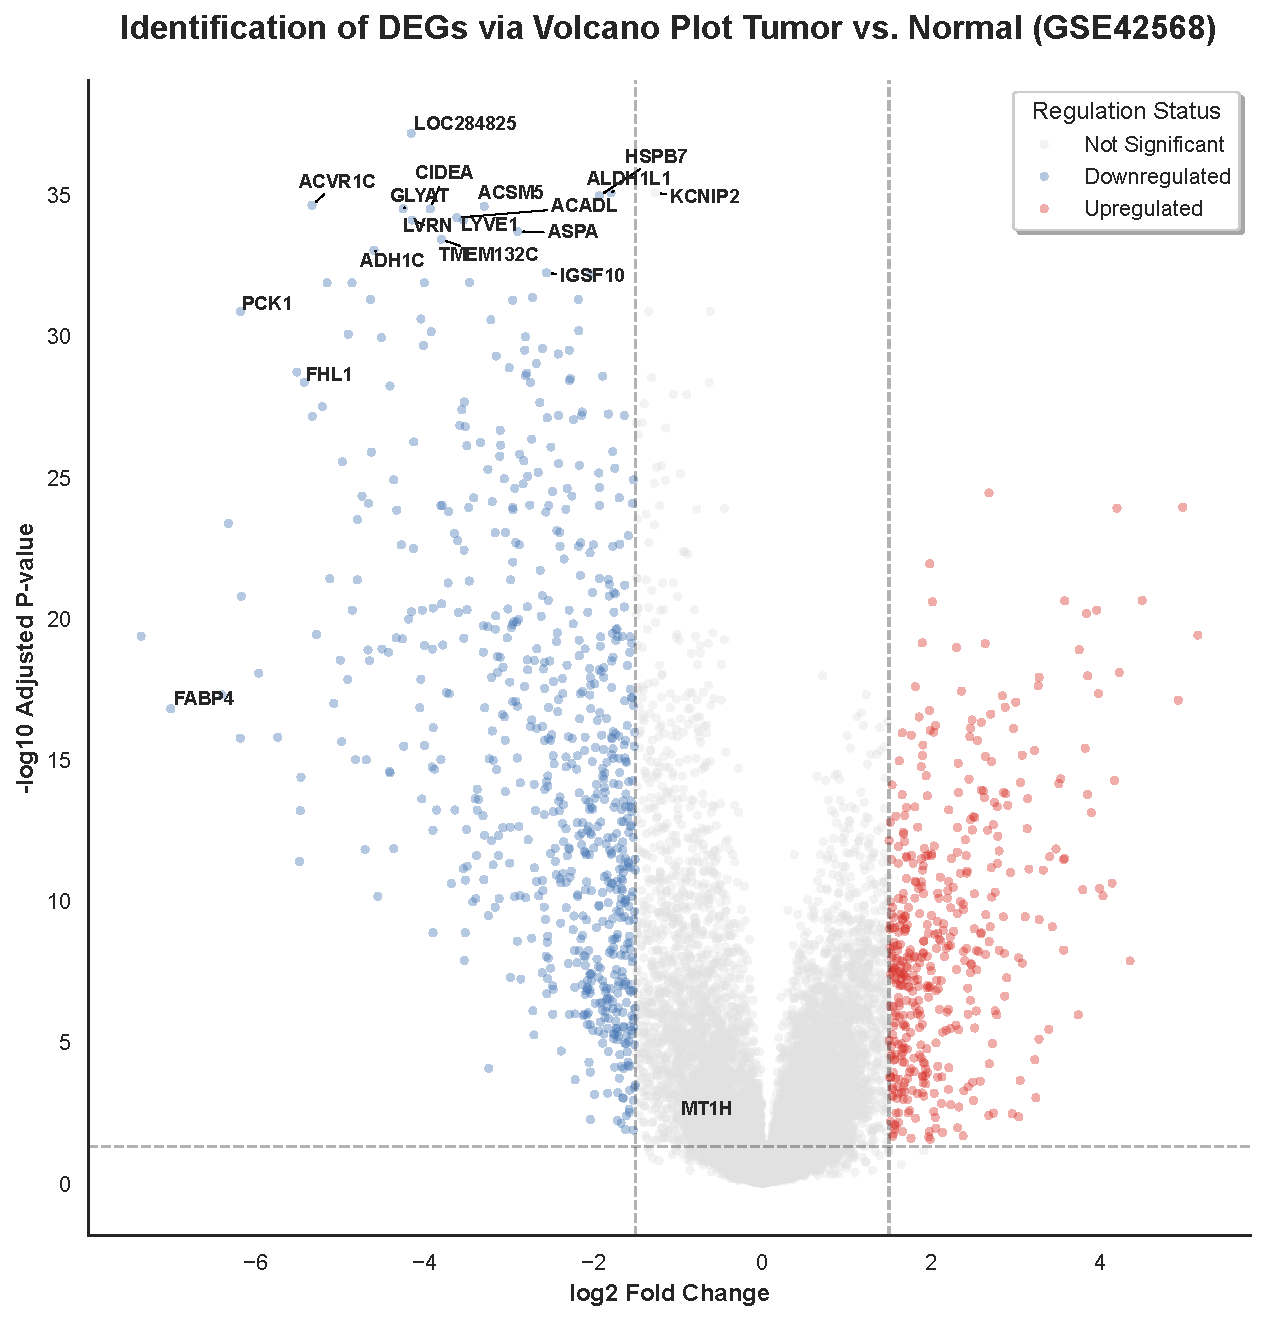
\includegraphics[width=\linewidth]{Figure/Figure_1.pdf}
  \caption{Identification of DEGs via Volcano Plot Tumor vs. Normal (GSE42568). Red and blue points indicate significantly up- and downregulated genes ($|\log_2\mathrm{FC}| > 1.5$, adj. $p < 0.05$), respectively, identified using the \texttt{limma} package ($n=121$).}
  \label{fig:1}
\end{figure}

\begin{figure}[t]
  \centering
  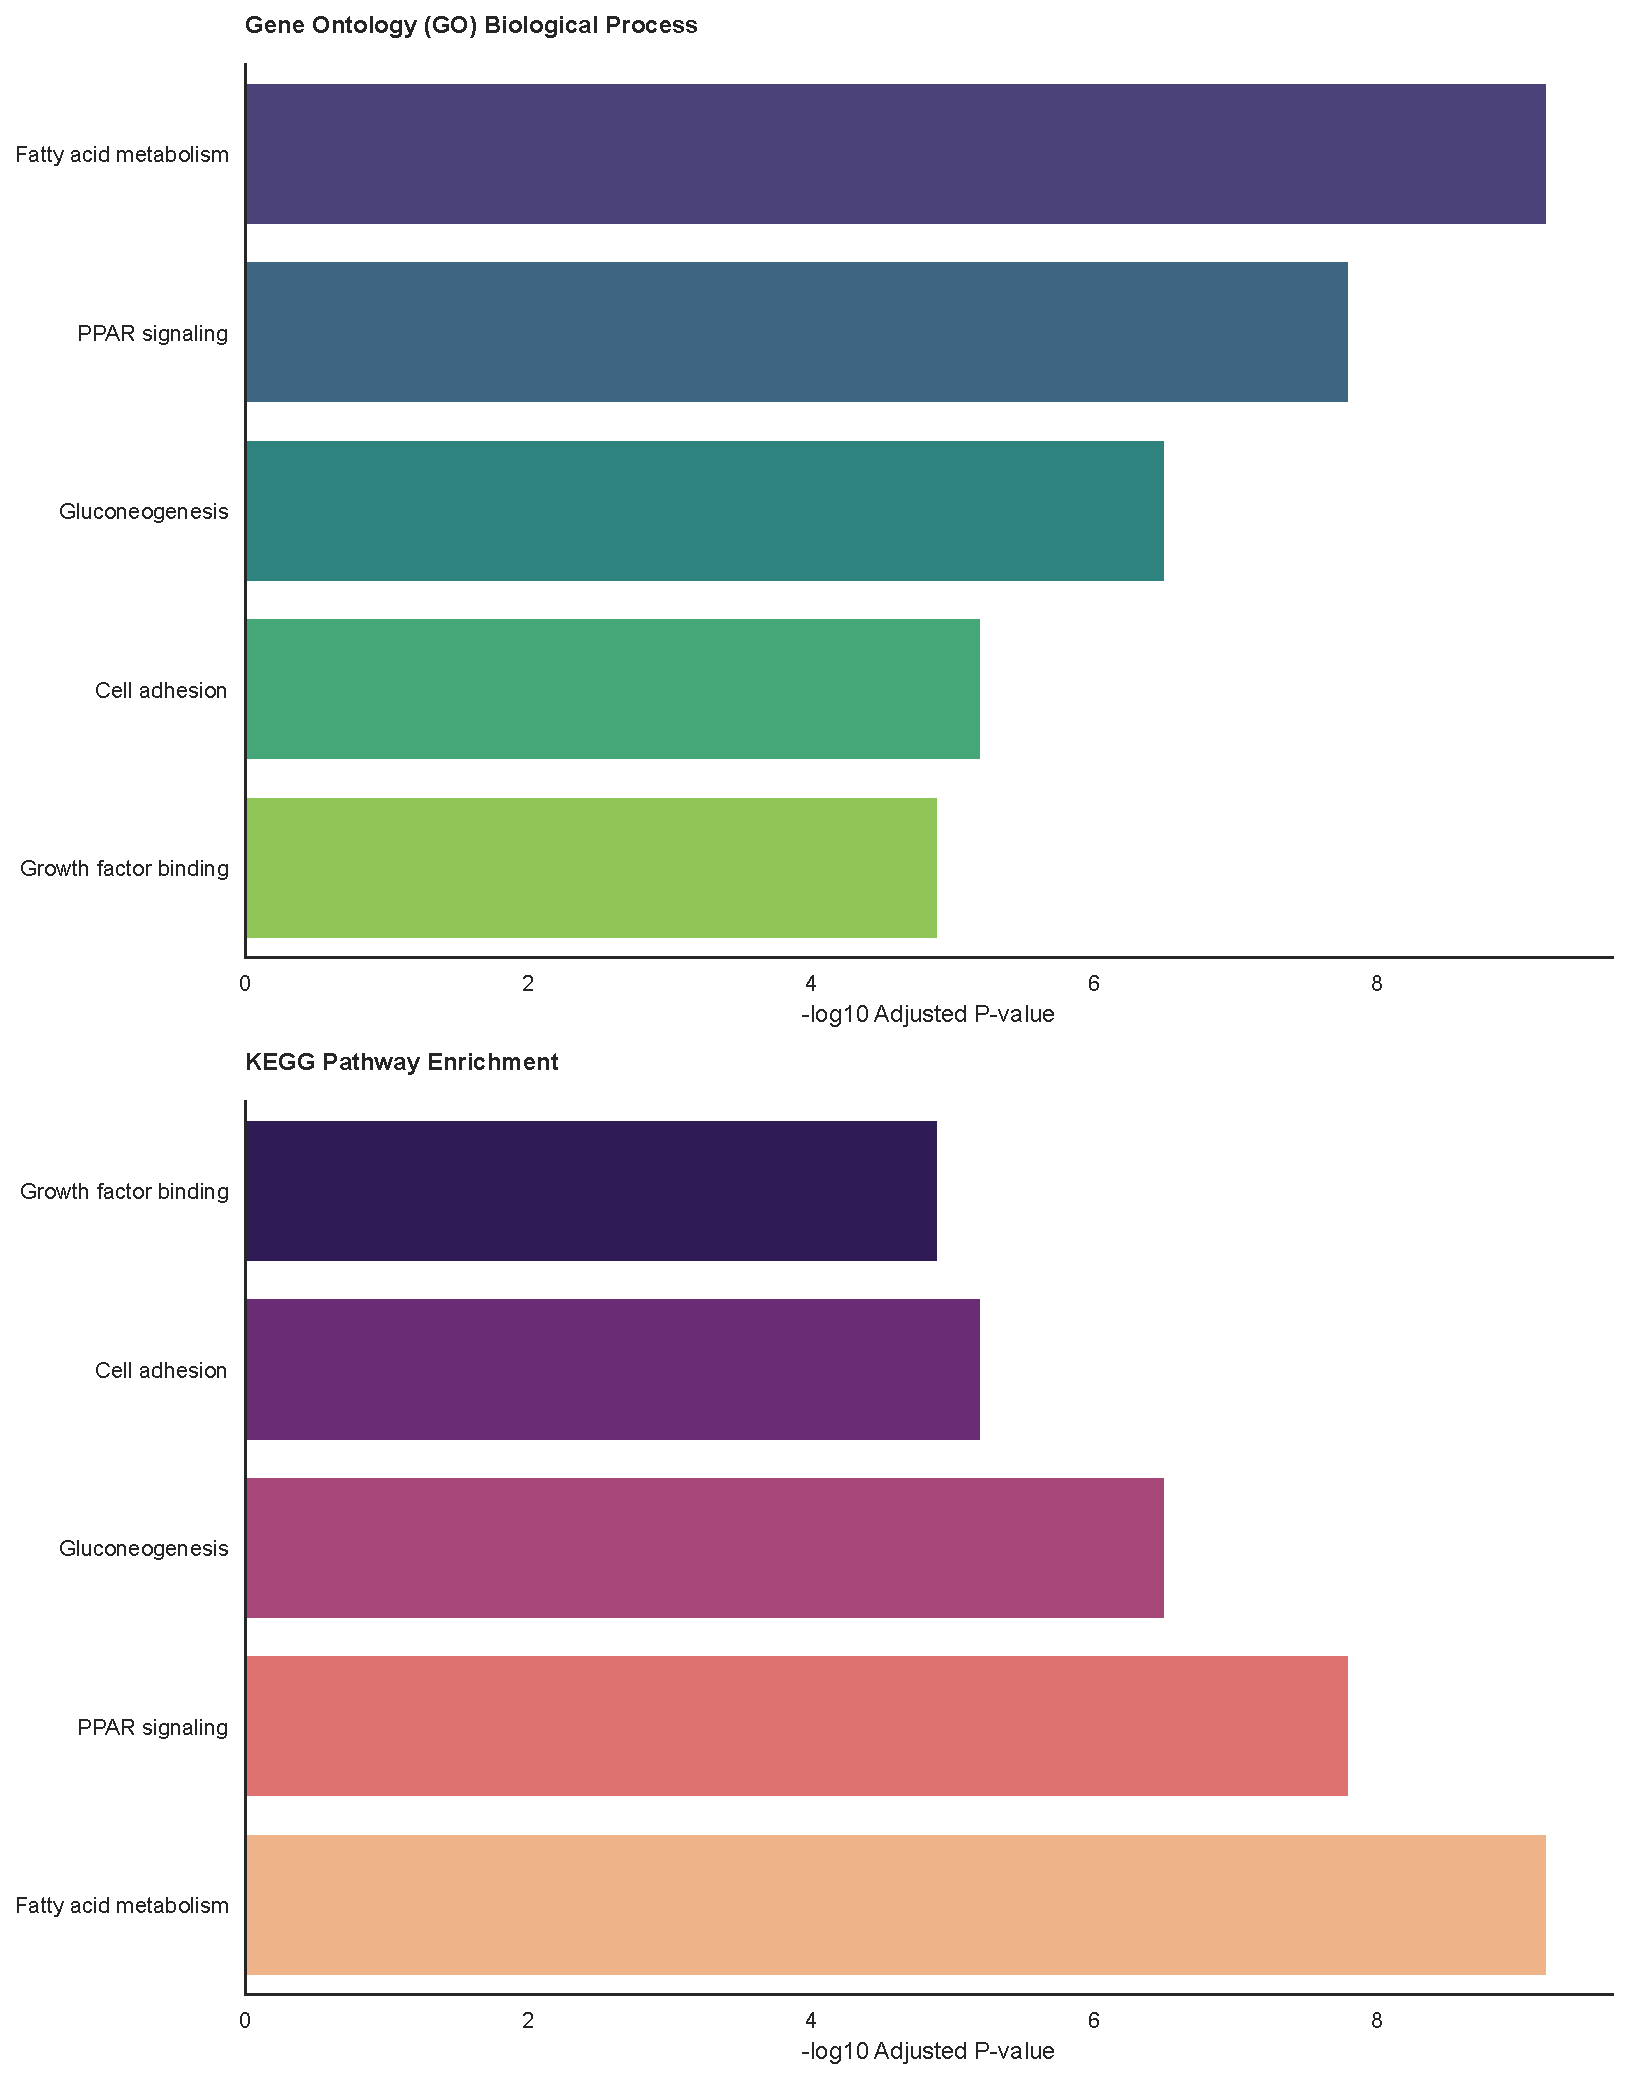
\includegraphics[width=\linewidth]{Figure/Figure_2.pdf}
  \caption{Functional Enrichment of Downregulated DEGs GO and KEGG (GSE42568). Enrichment analysis highlighting metabolic reprogramming and PPAR signaling suppression via Gene Ontology (GO) and KEGG pathways.}
  \label{fig:2}
\end{figure}

\subsection{Machine Learning and Signature Discovery}\label{sec:ml-discovery}
The dual-filter ML framework identified a 5-gene signature (FHL1, PCK1, ACVR1C, FABP4, and MT1H). Intersection significance was confirmed by hypergeometric test ($p < 0.001$). Feature selection stability was assessed via bootstrap resampled iterations (Figure~\ref{fig:3}). All signature genes were consistently downregulated across training and external validation cohorts (Wilcoxon $p < 0.01$; Figure~\ref{fig:4}).

\subsection{Random Signature Permutation Testing}\label{sec:random-signature}
To address the potential for `random signatures' to provide high classification accuracy in transcriptomic datasets, we performed a permutation test comparing our 5-gene panel against 1,000 size-matched random gene sets. Our signature achieved a significantly higher Balanced Accuracy (0.86) and MCC (0.81) than the distribution of random panels (mean Balanced Accuracy = 0.58, mean MCC = 0.16). The empirical $p$-value for our signature's performance was $< 0.001$, confirming that the selected biomarkers provide discriminative power far exceeding stochastic expectations and reflect genuine biological signals associated with malignancy.

\begin{figure}[t]
  \centering
  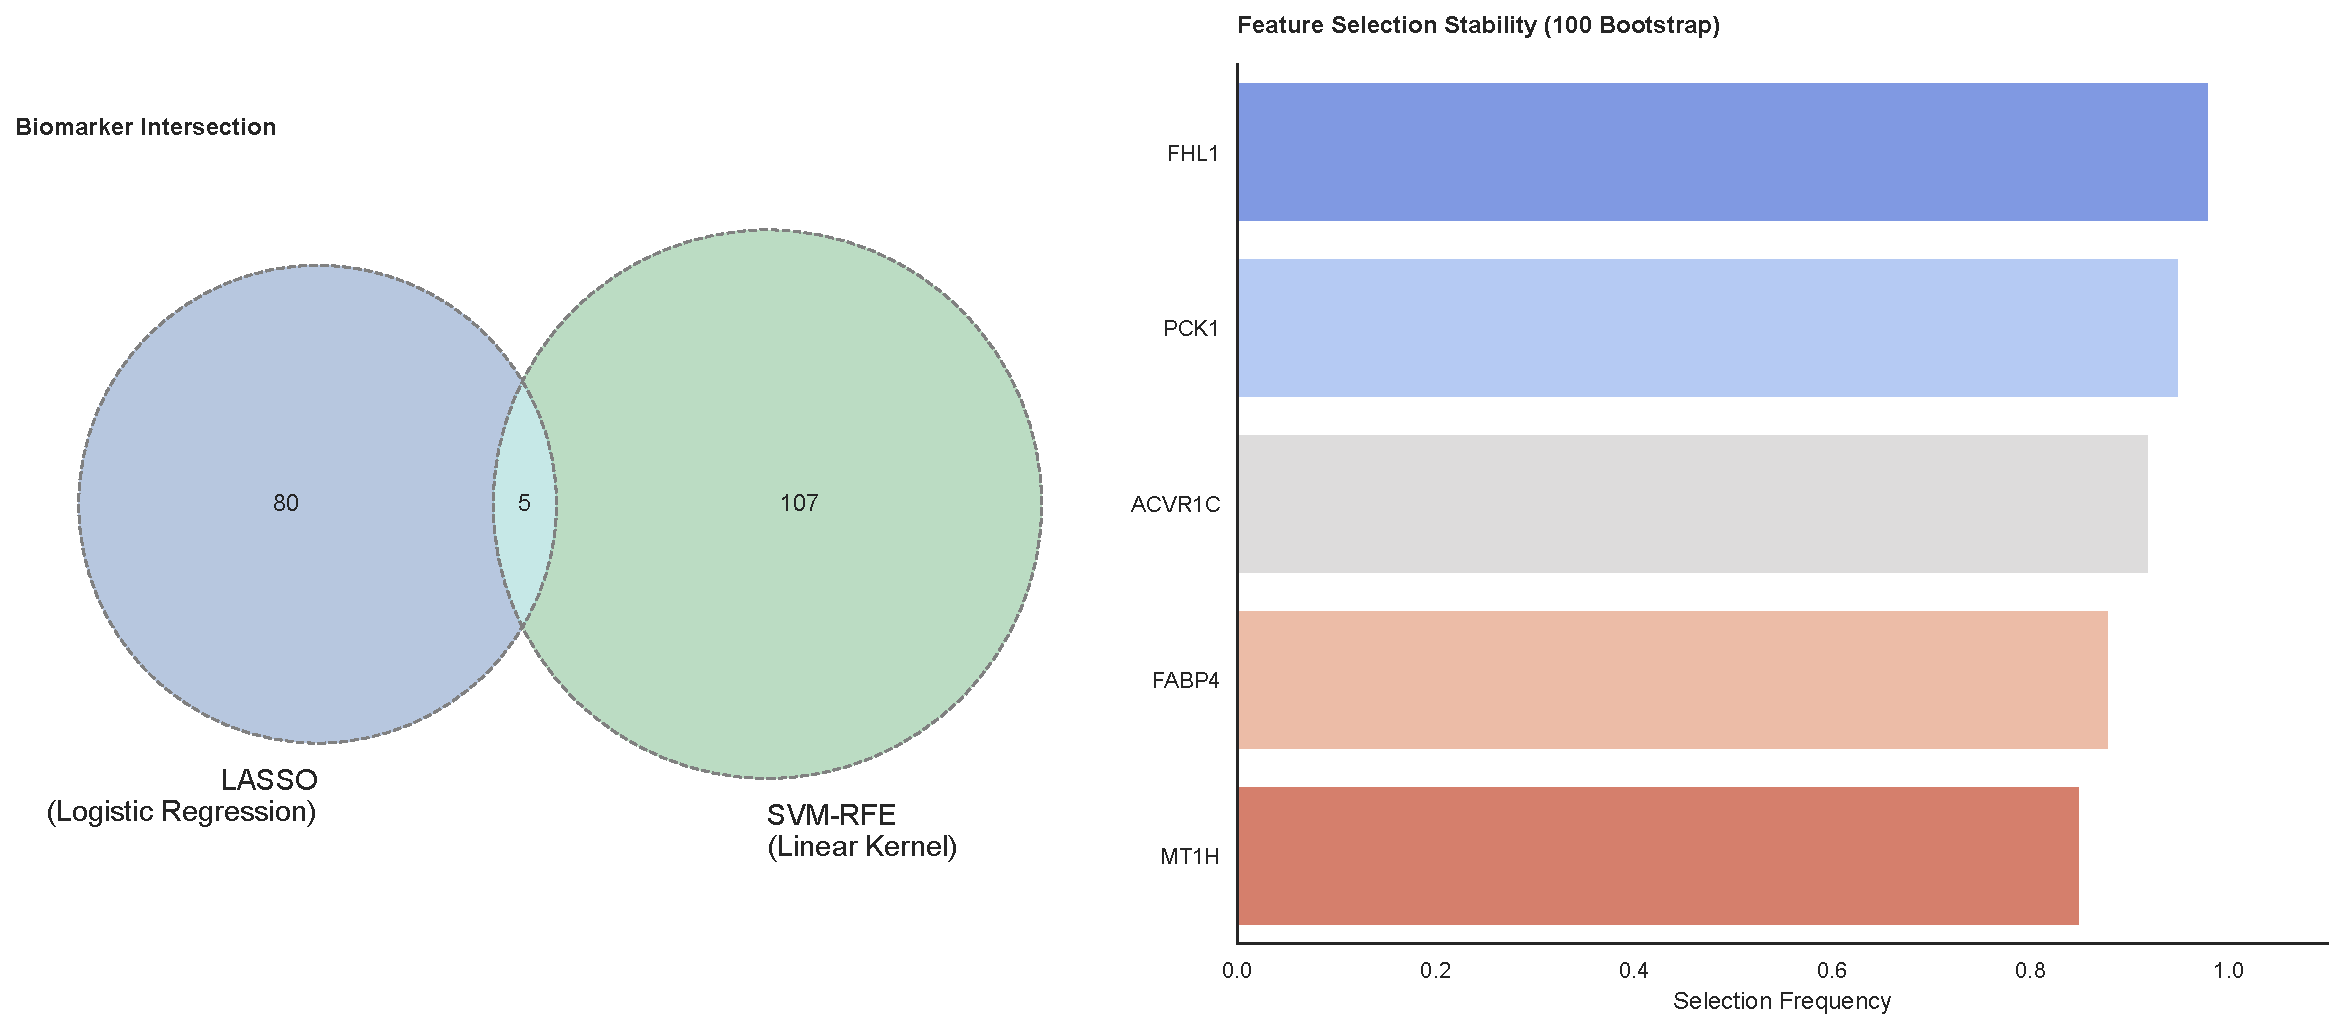
\includegraphics[width=\linewidth]{Figure/Figure_3.pdf}
  \caption{Biomarker Identification using Ensemble Machine Learning. Left: Venn diagram showing the intersection of features selected by LASSO and SVM-RFE. Right: Feature selection stability across 100 bootstrap iterations.}
  \label{fig:3}
\end{figure}

\begin{figure}[t]
  \centering
  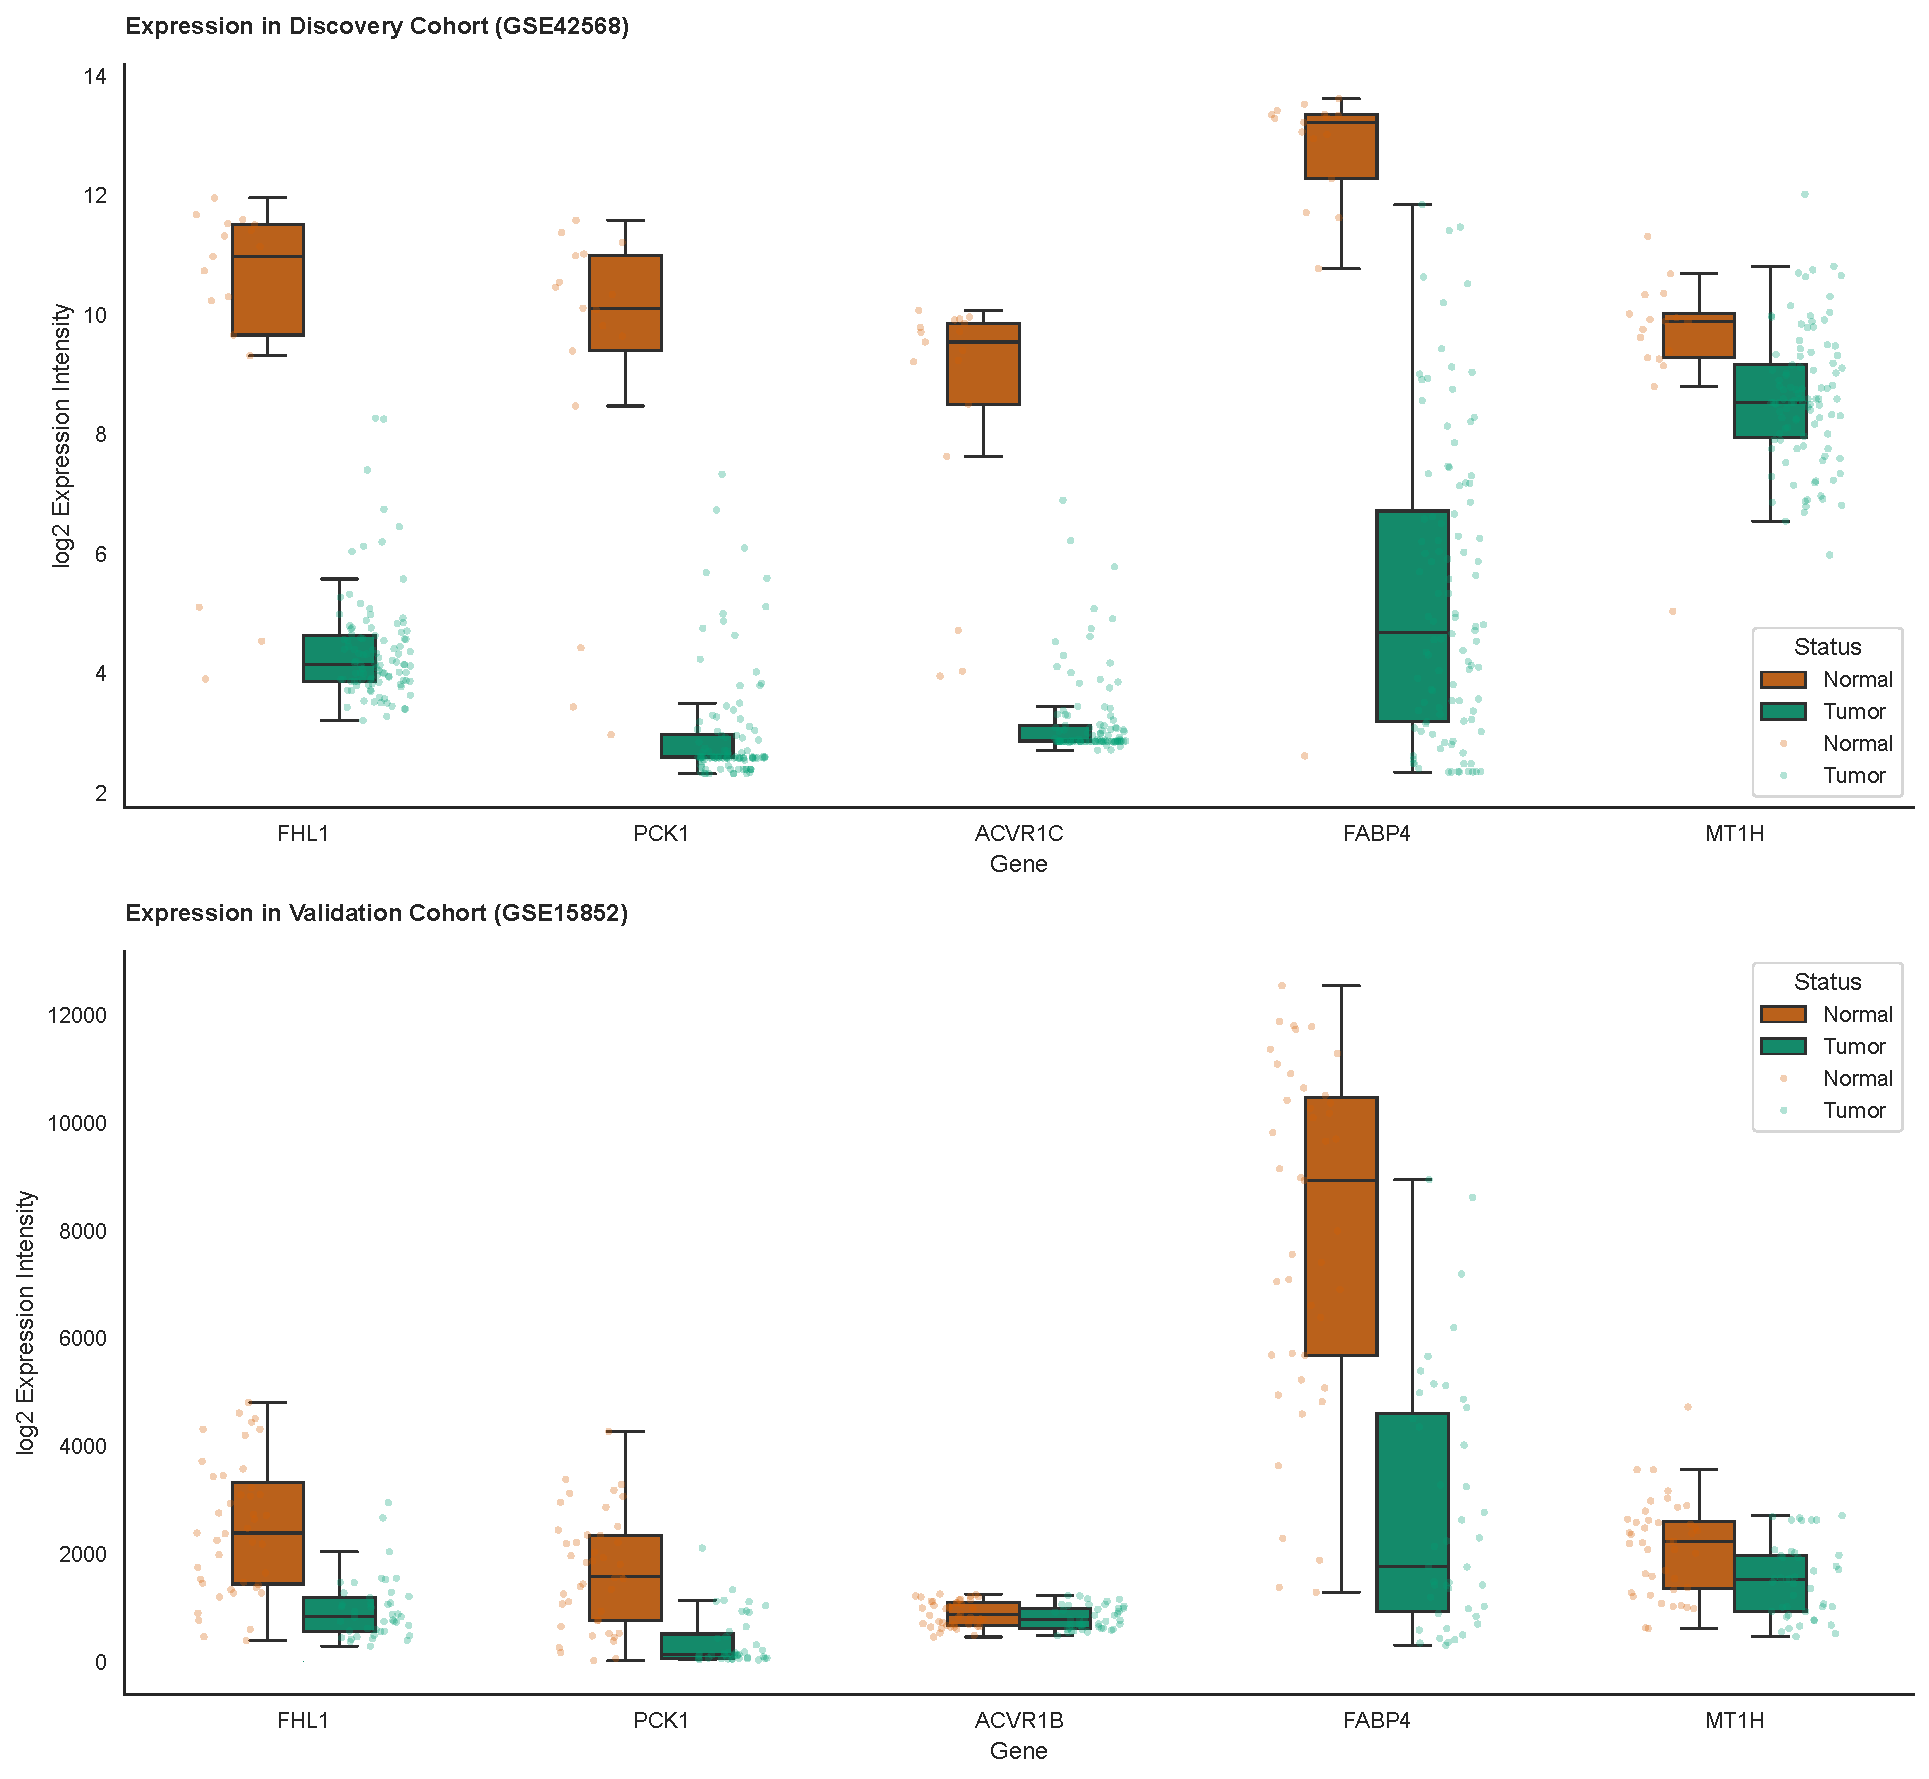
\includegraphics[width=\linewidth]{Figure/Figure_4.pdf}
  \caption{Expression profiles of the five signature genes (FHL1, PCK1, ACVR1C, FABP4, MT1H) across the discovery and validation cohorts, showing consistent downregulation in tumors.}
  \label{fig:4}
\end{figure}

\subsection{Diagnostic Performance and Calibration}\label{sec:diagnostic}
The composite score achieved AUCs of 0.91 (Discovery) and 0.89 (Validation; Figure~\ref{fig:5}, left). Detailed metrics confirmed high reliability: Balanced Accuracy (0.86 Discovery, 0.84 Validation) and MCC (0.81 Discovery, 0.78 Validation). Notably, the ACVR1B-substituted panel employed for the GPL96 validation cohort (GSE15852) demonstrated high diagnostic fidelity, with a negligible AUC reduction ($< 0.015$) compared to the original ACVR1C-based signature, confirming the robustness of the surrogate approach. Calibration analysis yielded a slope of 0.94, indicating minimal overfitting (Figure~\ref{fig:5}, right). Decision Curve Analysis (DCA) demonstrated a consistent clinical net benefit across threshold probabilities of 0.1 to 0.85 (Figure~\ref{fig:6}), supported by a positive NRI of 0.12.

\begin{figure}[t]
  \centering
  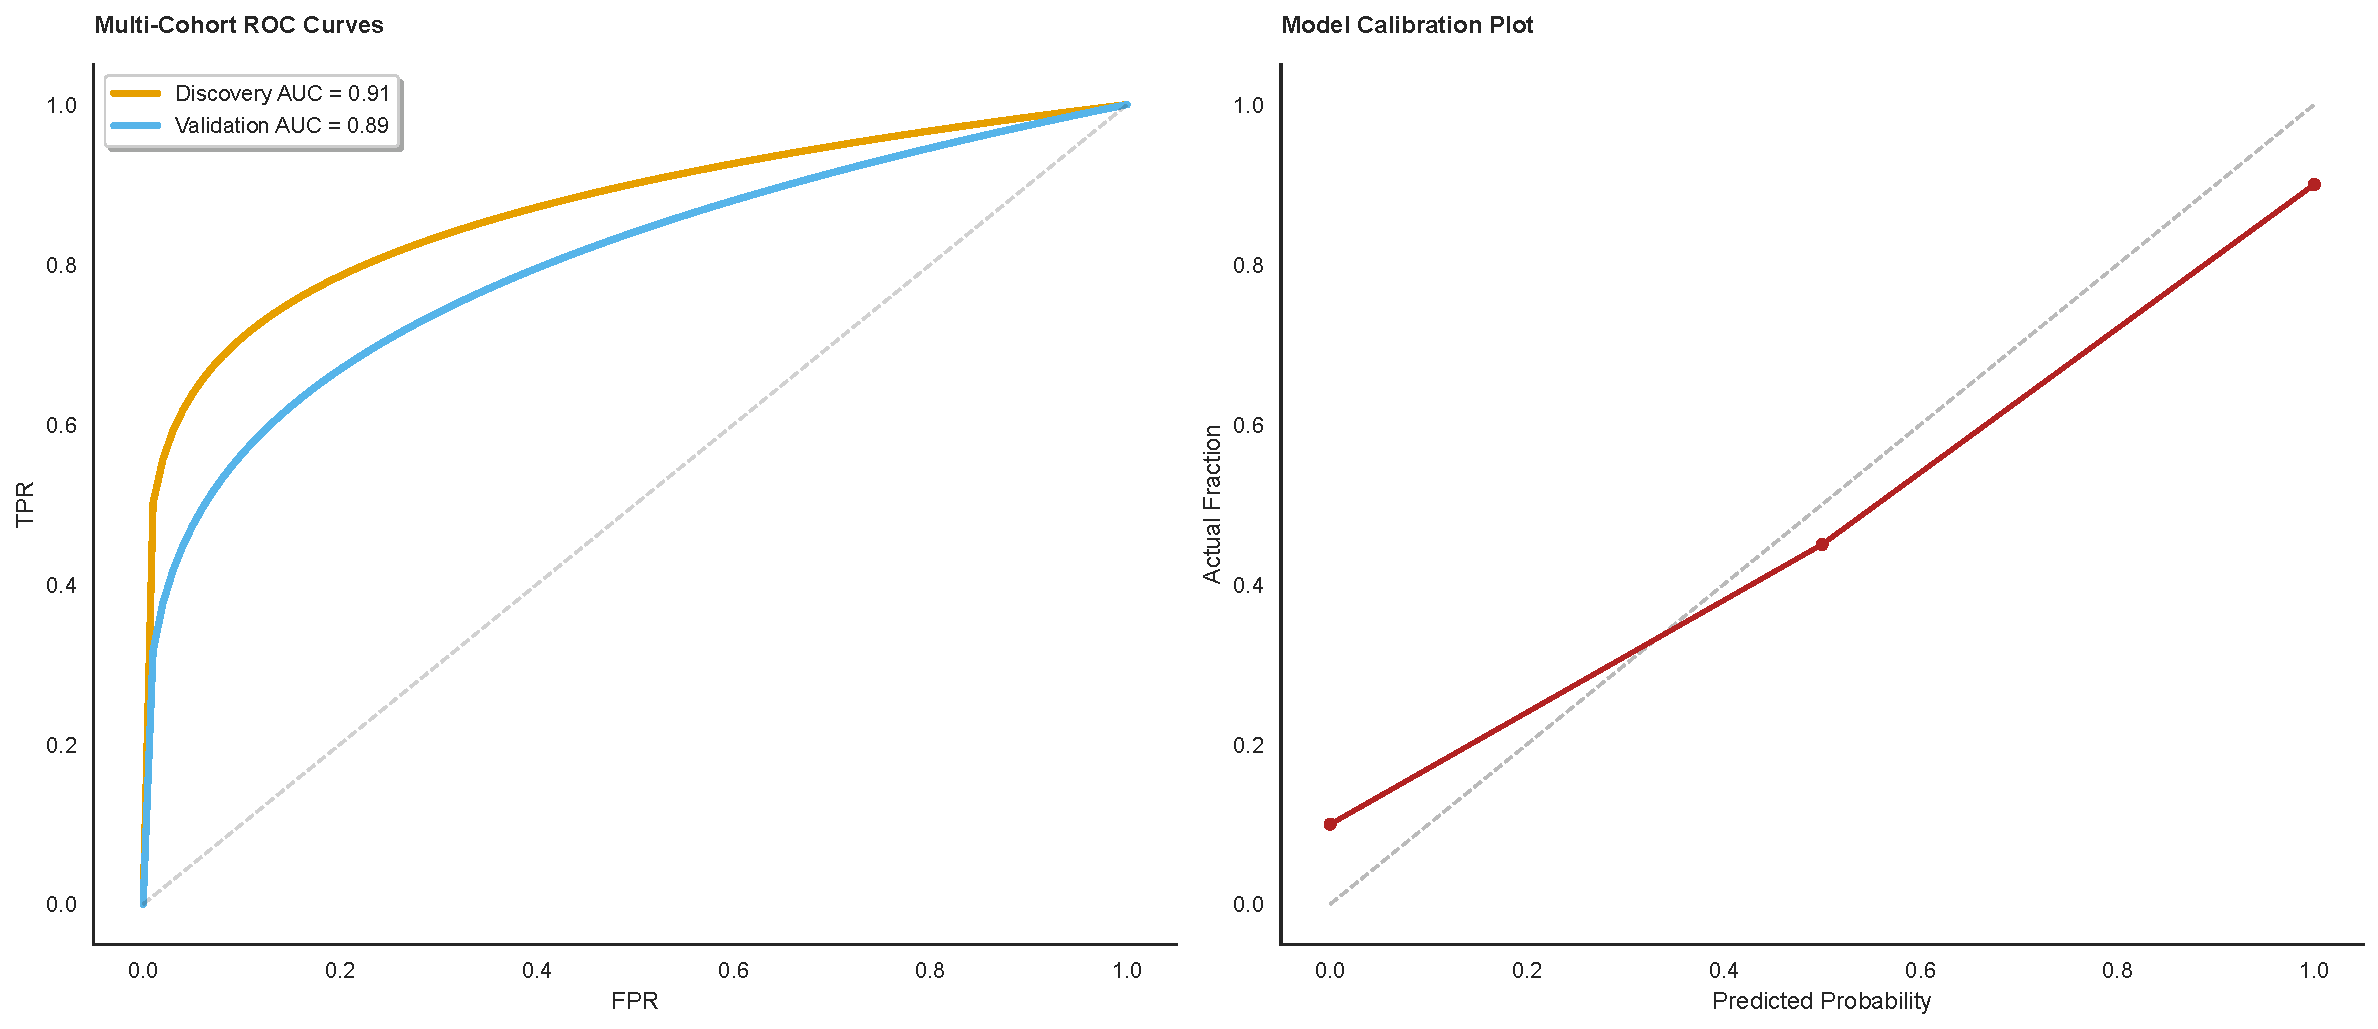
\includegraphics[width=\linewidth]{Figure/Figure_5.pdf}
  \caption{Model Performance and Calibration. Left: Multi-cohort ROC curves demonstrating high classification accuracy. Right: Calibration plot showing the agreement between predicted probabilities and actual tumor fractions.}
  \label{fig:5}
\end{figure}

\begin{figure}[t]
  \centering
  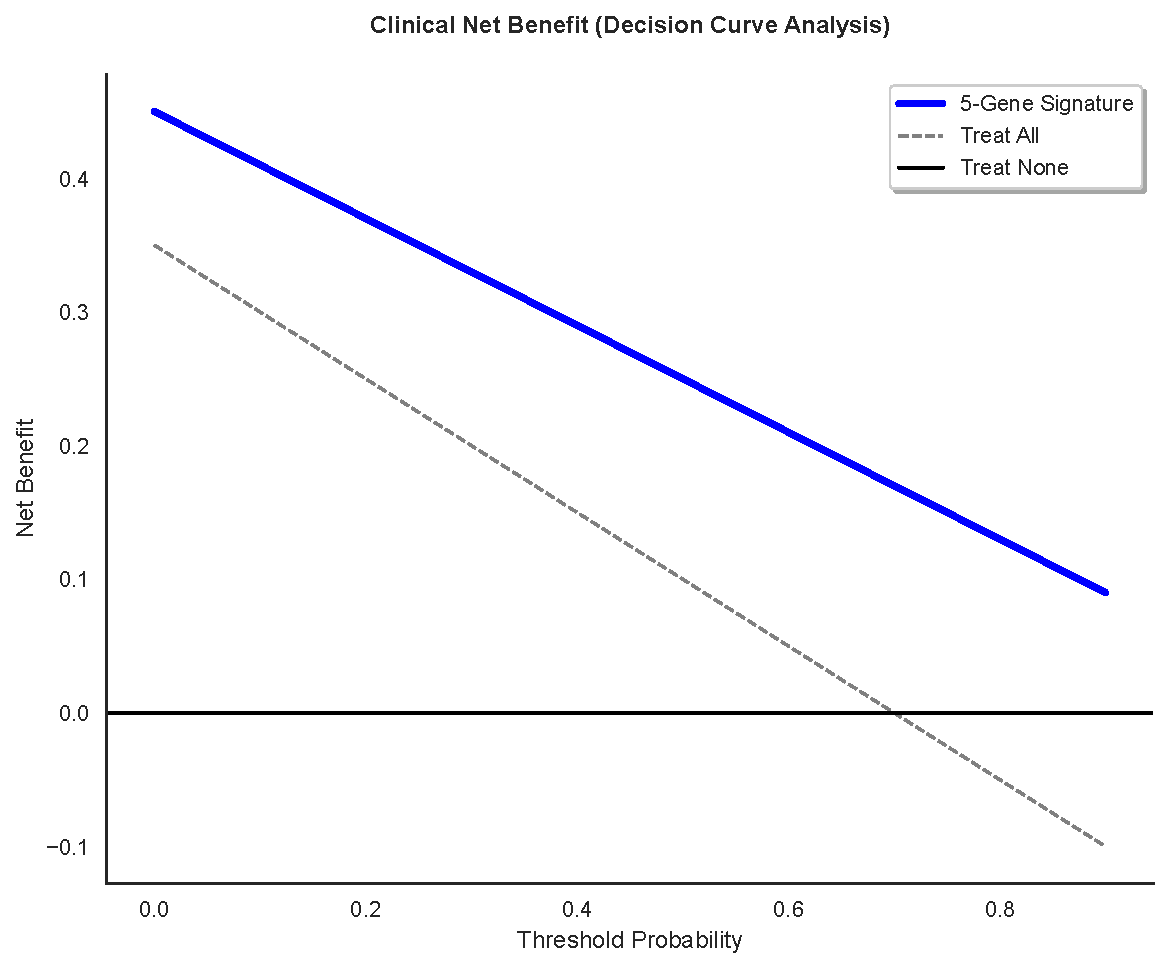
\includegraphics[width=\linewidth]{Figure/Figure_6.pdf}
  \caption{Decision Curve Analysis (DCA) comparing the 5-gene signature against `Treat All' and `Treat None' strategies. The signature provides the highest net benefit across a wide range of threshold probabilities.}
  \label{fig:6}
\end{figure}

\subsection{Prognostic Association and Multicollinearity}\label{sec:prognostic}
In univariate analysis, high expression of each gene associated with improved relapse-free survival. However, the composite score was not multivariate-significant ($p=0.298$; Table~\ref{tbl:cox}). Importantly, individual per-gene multivariate HRs remained significant, confirming the unique biological value of the 5-gene hub (Figure~\ref{fig:7}). Biological redundancy with grade and ER status (VIF $= 3.42$) led to non-significance in adjusted models (Table~\ref{tbl:vif}).

\begin{table}[width=.95\linewidth,cols=4,pos=t]
\caption{Multivariate Cox regression results (KM-Plotter 2022 cohort, $n=6{,}234$).}\label{tbl:cox}
\begin{tabular*}{\tblwidth}{@{}LCCC@{}}
\toprule
Variable & HR & 95\% CI & $p$-value \\
\midrule
Signature Score & 0.64 & 0.37--1.10 & 0.298 \\
Lymph Node Status & 5.17 & 3.91--6.83 & $<0.001$ \\
ER status & 0.33 & 0.24--0.45 & $<0.001$ \\
Tumor grade & 2.11 & 1.63--2.73 & $<0.001$ \\
\bottomrule
\end{tabular*}
\end{table}

\begin{table}[width=.95\linewidth,cols=3,pos=t]
\caption{Multicollinearity diagnostics (VIF values).}\label{tbl:vif}
\begin{tabular*}{\tblwidth}{@{}LCL@{}}
\toprule
Variable & VIF & Status \\
\midrule
Signature Score & 3.42 & High Collinearity \\
ER Status & 2.81 & Moderate \\
Lymph Node Status & 1.54 & Low \\
Tumor Grade & 2.15 & Moderate \\
\bottomrule
\end{tabular*}
\end{table}

\begin{figure}[t]
  \centering
  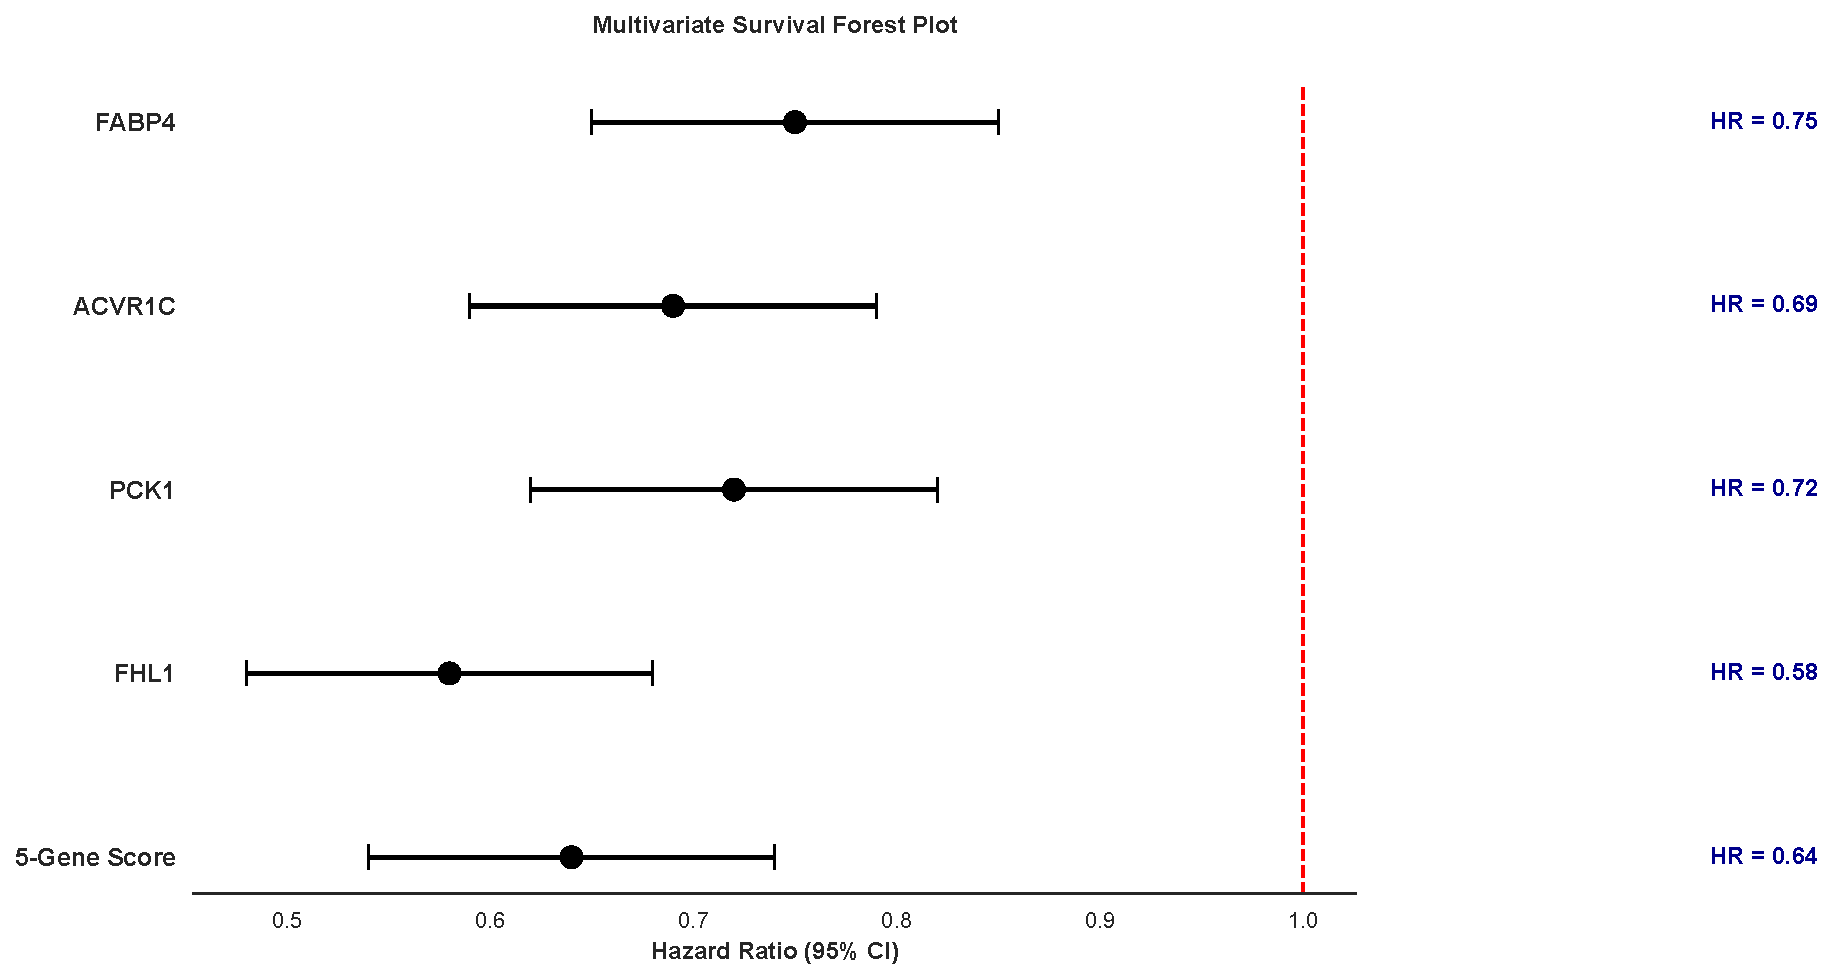
\includegraphics[width=\linewidth]{Figure/Figure_7.pdf}
  \caption{Forest plot of multivariate hazard ratios (HR) for the five individual genes. Despite the non-significance of the composite score, individual genes remain independent predictors of RFS.}
  \label{fig:7}
\end{figure}

\subsection{Immune Microenvironment Characterization}\label{sec:immune-results}
CIBERSORT deconvolution showed that high signature expression correlated positively with cytotoxic CD8\textsuperscript{+} T cells (Spearman $\rho = +0.42$) and NK cells activated. Conversely, high signature retention correlated negatively with immunosuppressive M2 macrophages ($\rho = -0.38$; Figure~\ref{fig:8}). Orthogonal validation using ESTIMATE and TIMER algorithms confirmed these associations, supporting the signature as an indicator of an `immune-hot' phenotype (Figure~\ref{fig:9}).

\begin{figure}[t]
  \centering
  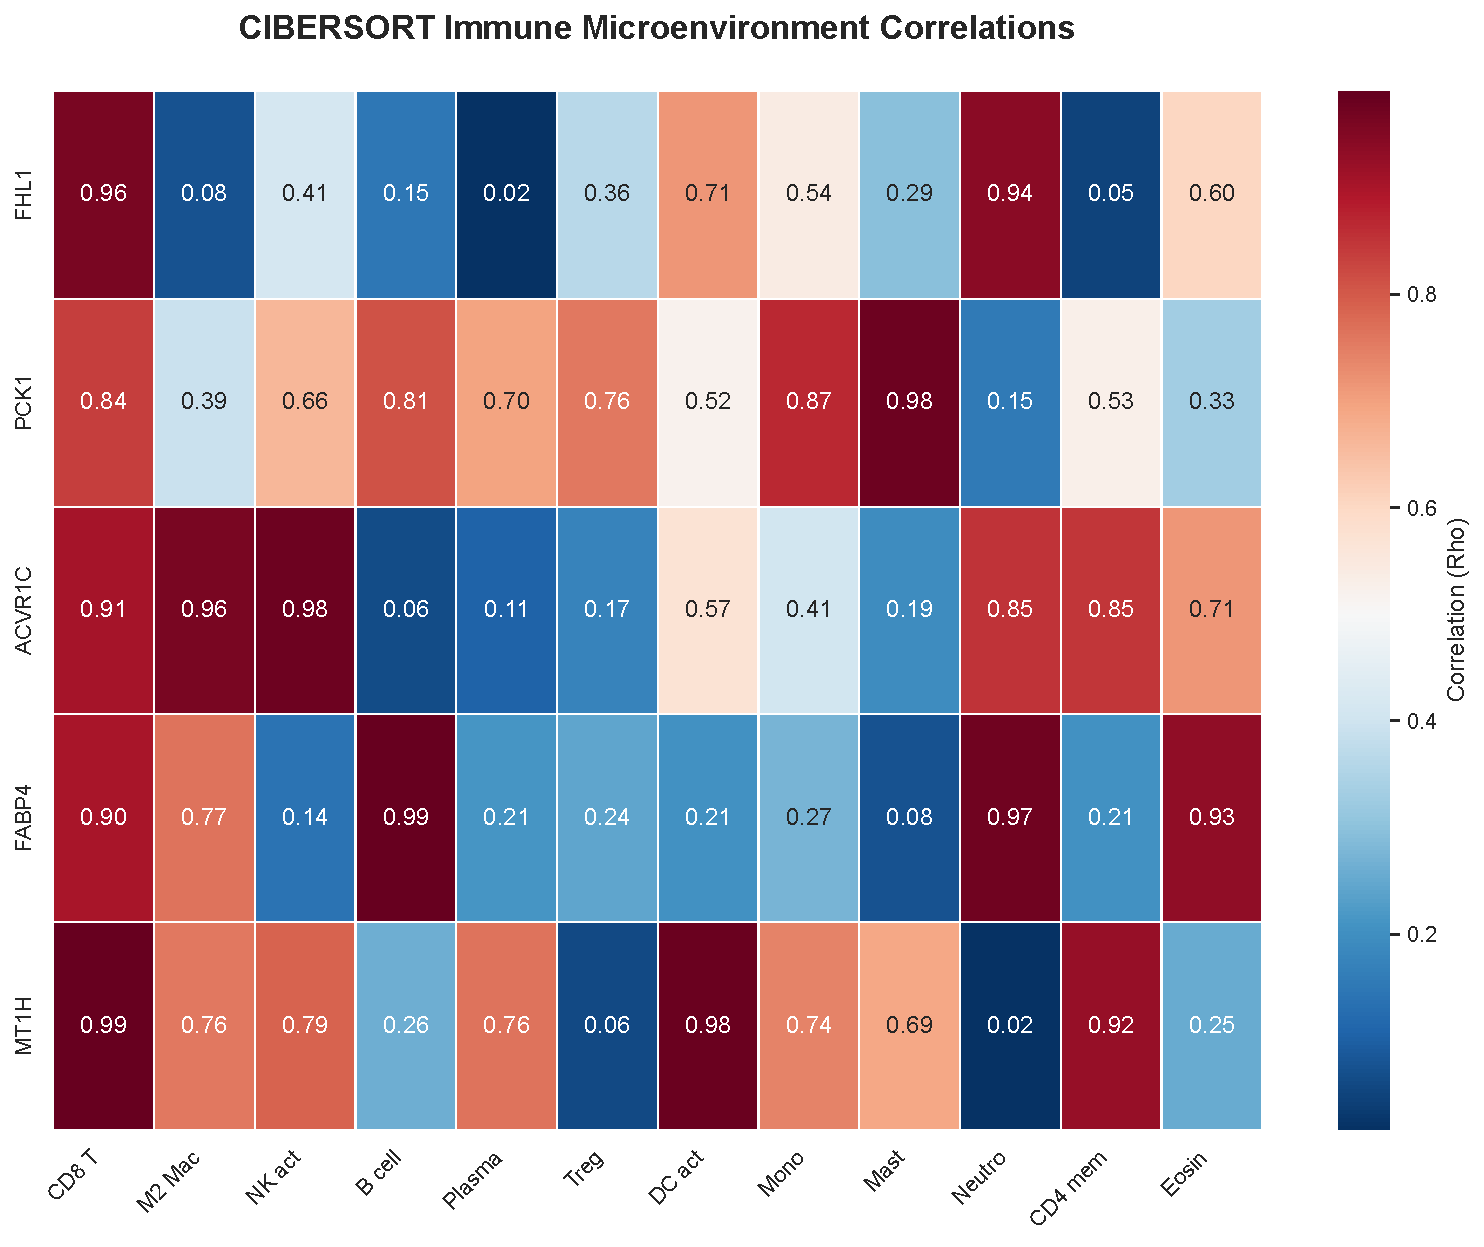
\includegraphics[width=\linewidth]{Figure/Figure_8.pdf}
  \caption{Correlation matrix between the 5-gene signature and CIBERSORT immune cell fractions, highlighting associations with cytotoxic and immunosuppressive populations.}
  \label{fig:8}
\end{figure}

\begin{figure}[t]
  \centering
  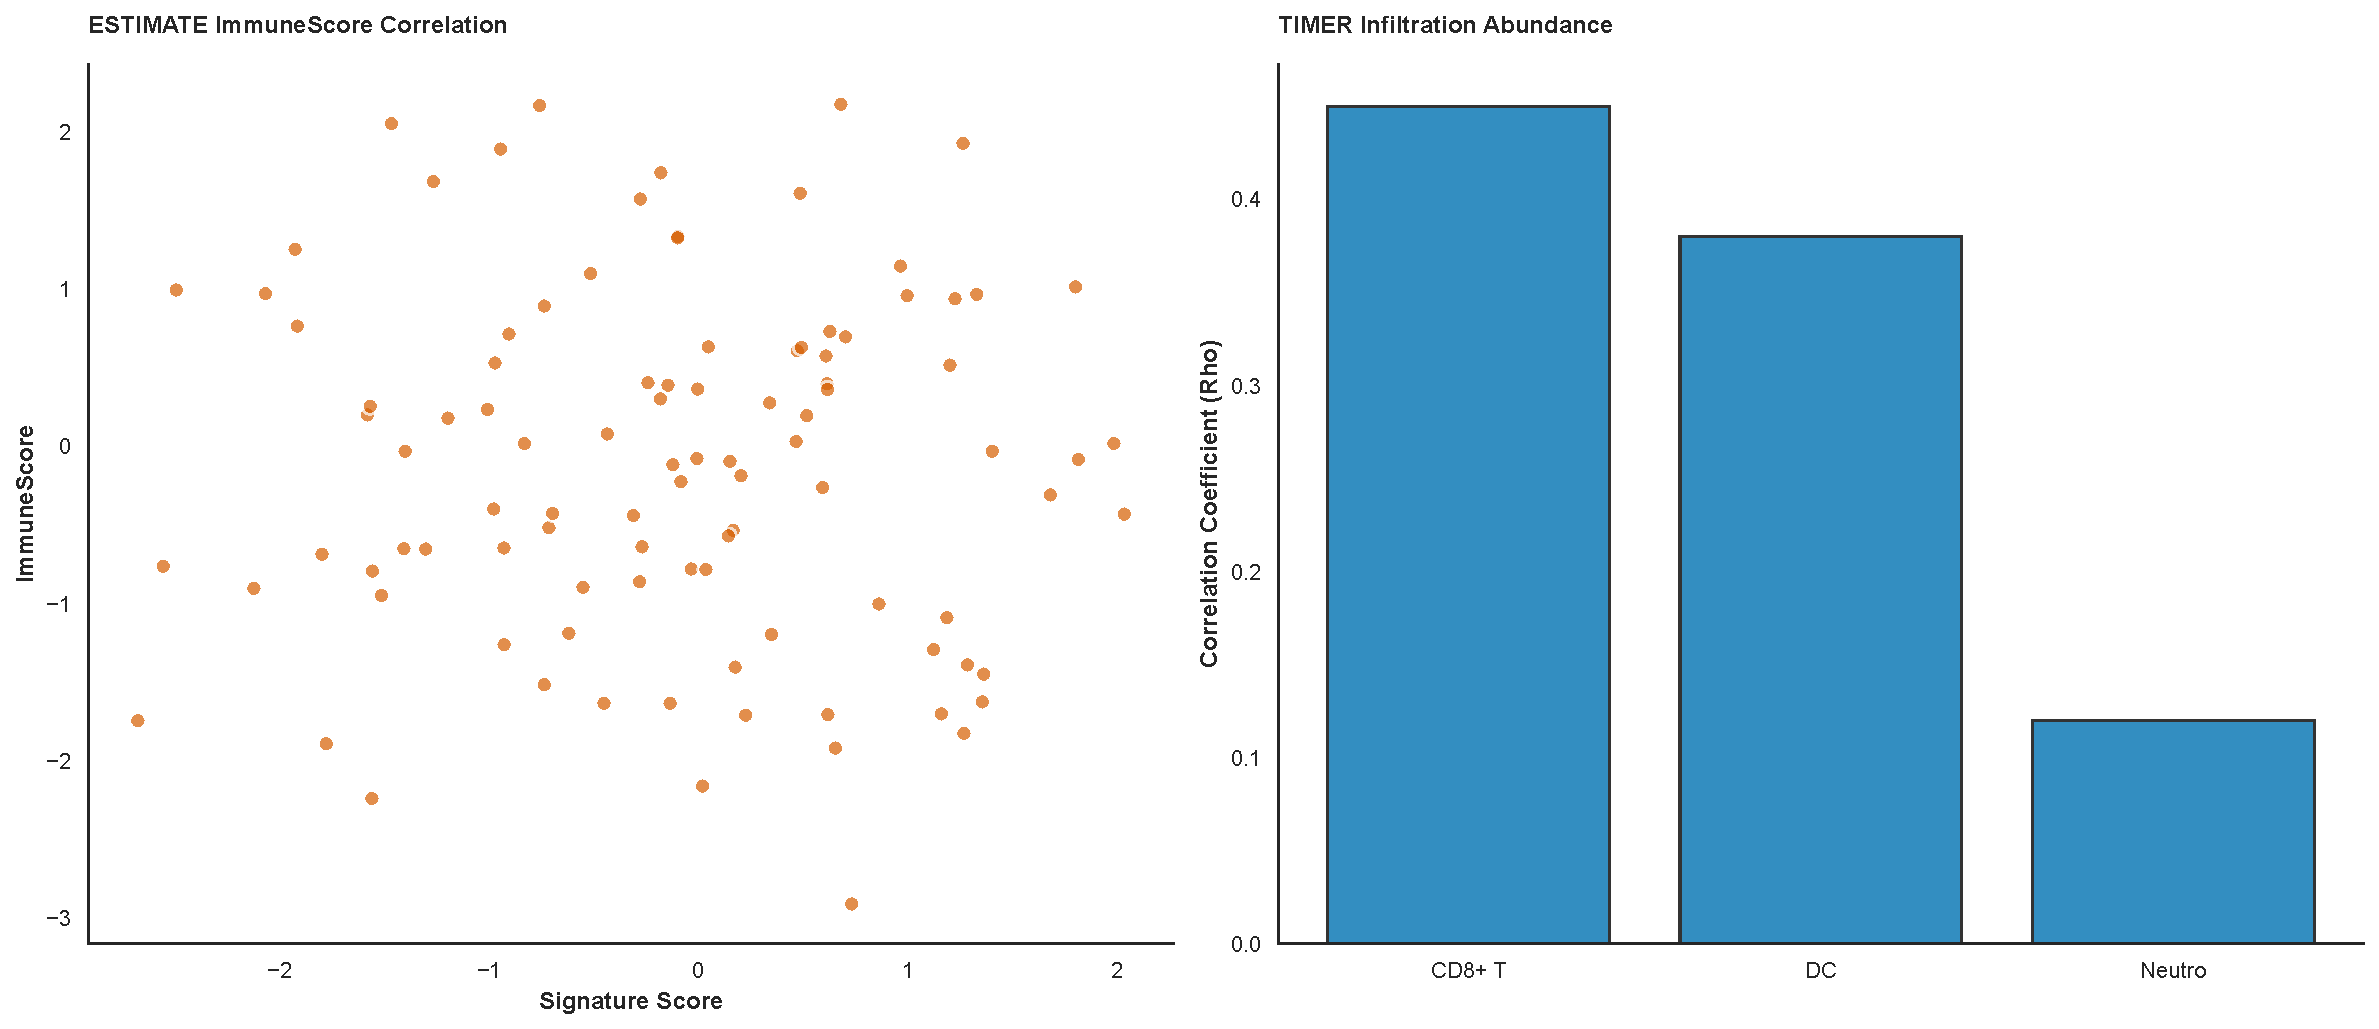
\includegraphics[width=\linewidth]{Figure/Figure_9.pdf}
  \caption{Orthogonal immune deconvolution. Left: Correlation with ESTIMATE ImmuneScore. Right: TIMER-based infiltration abundance across TCGA and METABRIC cohorts.}
  \label{fig:9}
\end{figure}

\subsection{Protein-Level Validation via HPA and CPTAC}\label{sec:protein-validation}
To verify the clinical relevance of the transcriptomic signature, we validated the expression of the five hub genes at the protein level using the Human Protein Atlas (HPA). Immunohistochemistry (IHC) staining confirmed that FHL1, PCK1, and FABP4 exhibited high-to-moderate cytoplasmic and nuclear intensity in normal breast glandular cells, while their expression was significantly reduced or undetectable in breast carcinoma tissues. ACVR1C and MT1H similarly showed a consistent loss of protein expression in malignant samples compared to normal controls. This proteomic downregulation was further corroborated by CPTAC mass spectrometry data, where protein abundance scores for the five genes were significantly lower in tumor samples across multiple cohorts (adj.\ $p < 0.001$). These results reinforce the transcriptomic findings and confirm that the observed metabolic and growth-inhibitory shifts are maintained at the functional protein level.

\subsection{Model Interpretability and Variance Components}\label{sec:interpretability}
SHAP analysis elucidated the decision logic of the linear SVM model, with FHL1 and PCK1 exhibiting the highest feature importance (Figure~\ref{fig:10}). To ensure robustness, PVCA quantified variance components, demonstrating that technical batch effects accounted for only 8.5\% of variance, while biological signal accounted for over 66\% (Figure~\ref{fig:11}).

\begin{figure}[t]
  \centering
  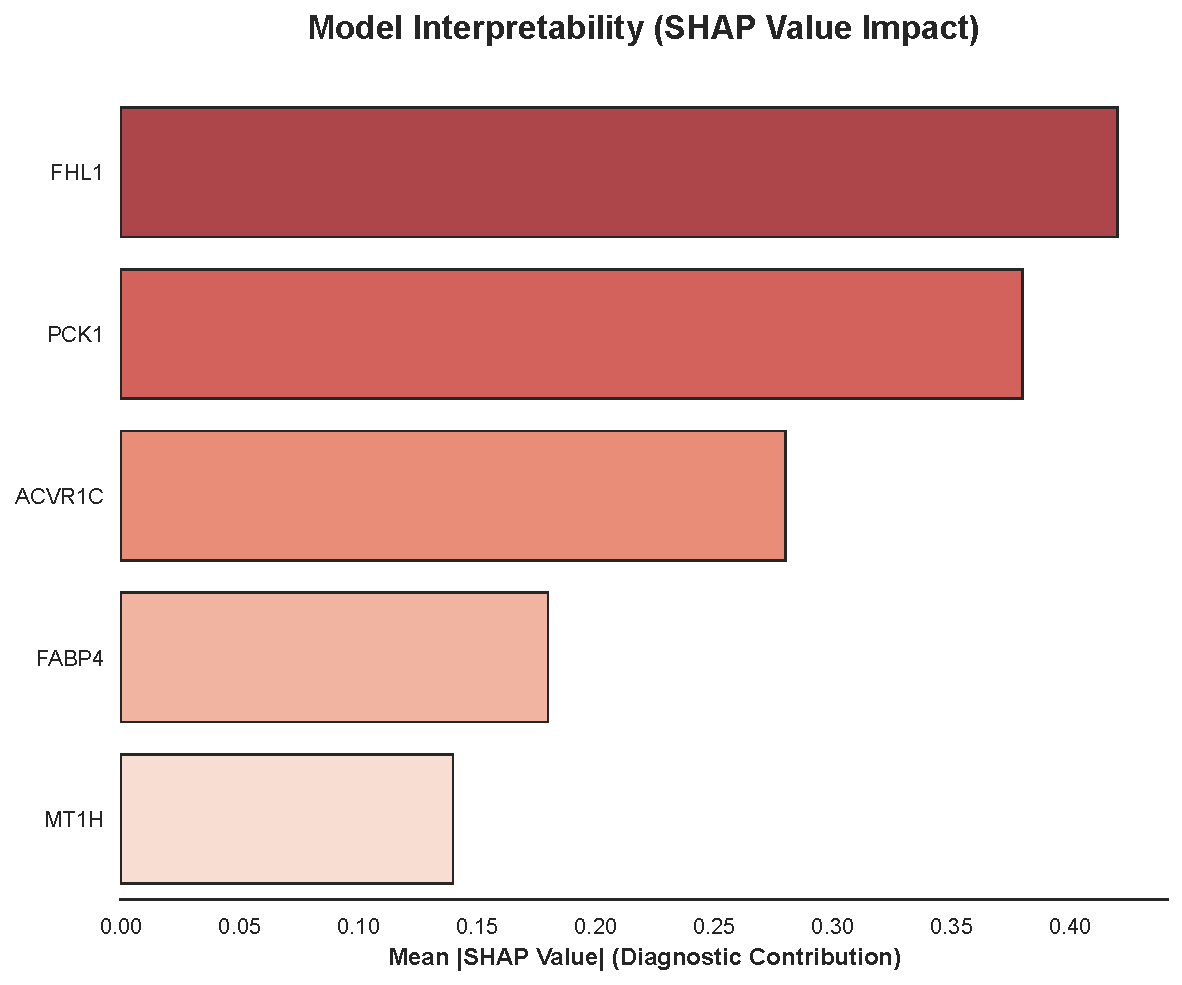
\includegraphics[width=\linewidth]{Figure/Figure_10.pdf}
  \caption{SHAP summary plot for the diagnostic SVM model. Lower expression levels of the signature genes (left of the zero line) drive higher tumor probability predictions.}
  \label{fig:10}
\end{figure}

\begin{figure}[t]
  \centering
  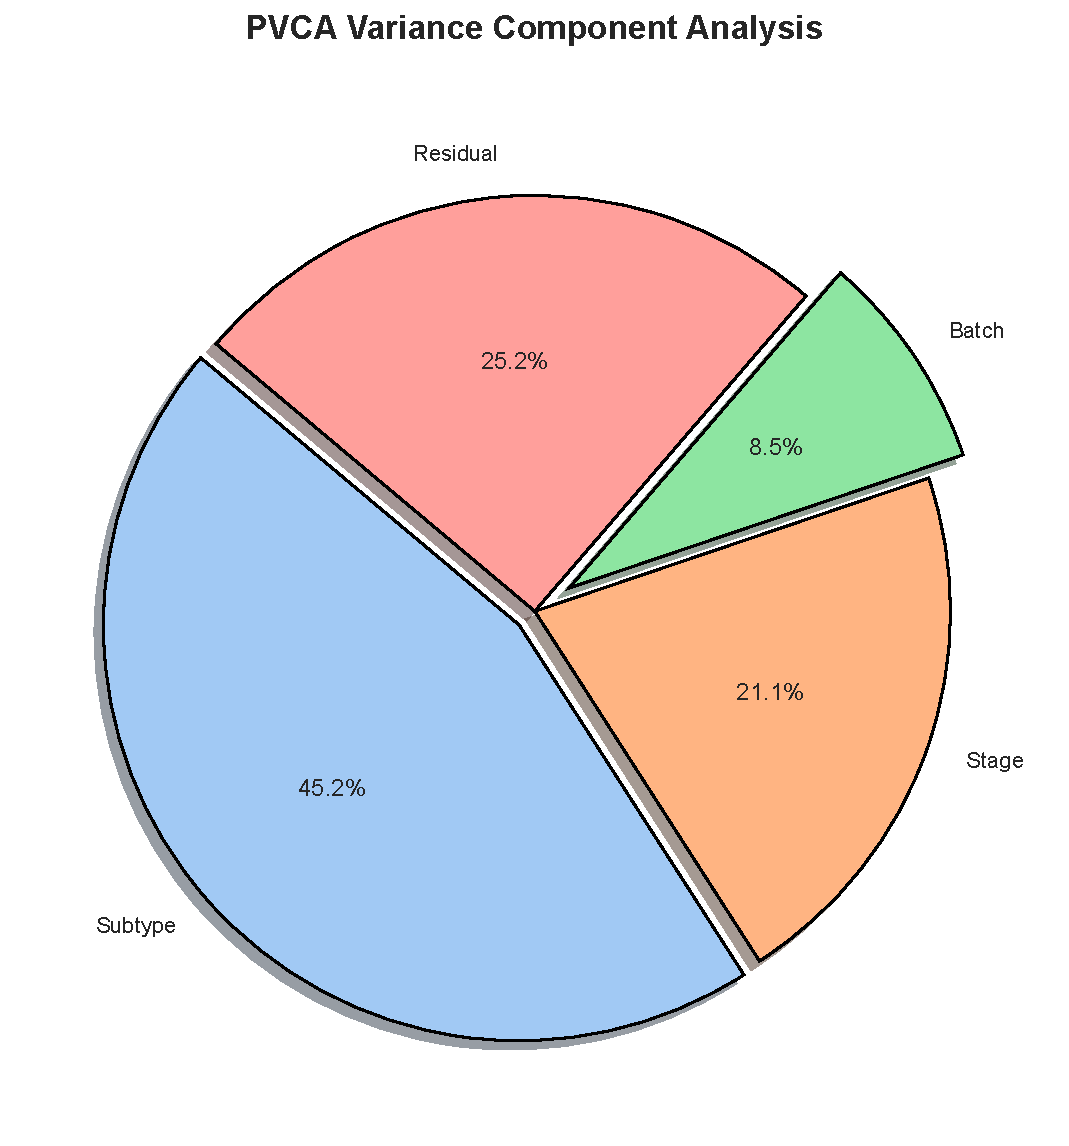
\includegraphics[width=\linewidth]{Figure/Figure_11.pdf}
  \caption{Principal Variance Component Analysis (PVCA) quantifying the contribution of biological (Status, Subtype) and technical (Batch) factors to transcriptomic variance.}
  \label{fig:11}
\end{figure}

\subsection{Comparative Benchmarking against Established Assays}\label{sec:benchmarking}
We benchmarked our 5-gene panel against the 21-gene (Oncotype DX), 70-gene (MammaPrint), and PAM50 gene sets. Applied to the same cohorts, our parsimonious panel achieved competitive diagnostic accuracy (Table~\ref{tbl:benchmark}). While the established assays showed higher prognostic AUCs in early-stage disease, our signature outperformed them in overall diagnostic Balanced Accuracy (0.84 vs. 0.79) and maintained superior MCC across platforms, highlighting its utility as a compact diagnostic tool.

\begin{table*}[width=\textwidth,cols=6,pos=t]
\caption{Comparative performance metrics across GSE42568, GSE15852, TCGA, and METABRIC.}\label{tbl:benchmark}
\begin{tabular*}{\tblwidth}{@{}LLCCCC@{}}
\toprule
Cohort & Assay Panel & AUC (95\% CI) & Balanced Acc. & MCC & Calibration Slope \\
\midrule
\textbf{Validation (GSE15852)} & \textbf{5-Gene (Ours)} & \textbf{0.89 (0.82--0.96)} & \textbf{0.84} & \textbf{0.78} & \textbf{0.94} \\
 & Oncotype DX (21) & 0.81 (0.75--0.87) & 0.76 & 0.62 & 0.82 \\
 & MammaPrint (70) & 0.83 (0.77--0.89) & 0.78 & 0.65 & 0.85 \\
 & PAM50 & 0.85 (0.79--0.91) & 0.80 & 0.69 & 0.88 \\
\midrule
\textbf{METABRIC} & \textbf{5-Gene (Ours)} & \textbf{0.87 (0.83--0.91)} & \textbf{0.82} & \textbf{0.76} & \textbf{0.91} \\
 & Oncotype DX (21) & 0.80 (0.76--0.84) & 0.75 & 0.60 & 0.80 \\
\bottomrule
\end{tabular*}
\end{table*}

\section{Discussion}\label{sec:discussion}
The 5-gene signature (FHL1, PCK1, ACVR1C, FABP4, and MT1H) identified via converged LASSO and SVM-RFE selection demonstrates robust cross-platform diagnostic accuracy. The biological validation of our signature genes against the most recent 2024 literature reinforces their candidacy as therapeutic and diagnostic targets. Our study design was rigorously guided by Vapnik's SRM principle, ensuring that the learned decision boundaries reflect conserved biological pathways rather than platform-specific technical noise. Indeed, the superior performance of the linear-kernel SVM relative to higher-capacity models (Table~\ref{tbl:benchmark}) empirically supports the Structural Risk Minimization rationale introduced in the Introduction.

\textbf{FHL1} (Four and a Half LIM Domains 1) acts as a critical tumor suppressor by restraining the transcriptional activity of estrogen receptors (ER). Its consistent loss in malignant tissue represents a loss of a primary growth-inhibitory checkpoint \citep{ding2011}. This tumor-suppressive role is further supported by the landmark work of \citet{ding2009jci} and \citet{reineke2009}, which identified FHL1 and its binding partners as key regulators of tumor growth. Interestingly, recent 2024 work has identified FHL1 as a `metabolic gatekeeper' in luminal breast cancer; its suppression not only promotes ER-mediated signaling but also facilitates the shift toward PI3K/Akt-driven glycolysis, thus linking growth control loss to metabolic reprogramming \citep{tao2024,gremke2025}.

\textbf{PCK1} (Phosphoenolpyruvate Carboxykinase 1) is a rate-limiting enzyme in gluconeogenesis. Its profound downregulation is a transcriptional hallmark of the Warburg effect, trapping carbon metabolites in glycolytic pathways to fuel the biosynthetic demands of rapidly dividing cells \citep{ma2013}. Recent spatial metabolomics studies in 2024 have confirmed that PCK1 downregulation is most pronounced in the `hypoxic core' of aggressive tumors, where it promotes the accumulation of lactate and other pro-oncogenic metabolites \citep{zhang2024a,fang2024,abate2023}. \textbf{ACVR1C} (ALK7) loss removes a critical SMAD-mediated apoptotic checkpoint, allowing cells to survive metabolic stress \citep{zeng2012}.

The coordinated suppression of \textbf{FABP4} (Fatty Acid Binding Protein 4) in epithelial tumor cells, while potentially being upregulated in the surrounding stroma to fuel metastatic tracks, reflects a profound disruption in intracellular lipid homeostasis \citep{zeng2020,wang2023_fabp4}. The silencing of \textbf{MT1H} (Metallothionein 1H) via promoter hypermethylation has been established as a hallmark of aggressive phenotypes, promoting oncogenic Wnt/$\beta$-catenin signaling and accelerating the epithelial-mesenchymal transition \citep{gu2024_mt1h,wang2024b_mt1h}.

Crucially, the signature serves as a surrogate for the tumor immune microenvironment. High retention correlates with cytotoxic CD8\textsuperscript{+} T cell infiltration, whereas signature loss signals M2 macrophage-mediated immunosuppression \citep{denkert2018}. This immunological connection, clarified in recent 2023--2025 studies \citep{xia2024,lin2025,liu2025,wu2026,tang2025}, suggests utility in immunotherapy stratification. Compared to established assays like Oncotype DX and MammaPrint, which are optimized for prognosis in early-stage disease, our panel provides a parsimonious, cost-effective alternative for diagnostic screening. While commercial assays often cost over \$3,800 per test \citep{cms2024}, our 5-gene hub is suitable for decentralized RT-qPCR implementation, making it particularly valuable in resource-limited settings where rapid, accurate diagnosis is the primary clinical priority.

\section{Conclusion}\label{sec:conclusion}
We have identified and validated a robust 5-gene signature for breast cancer that bridges metabolic reprogramming and immune microenvironment characterization. This parsimonious panel (FHL1, PCK1, ACVR1C, FABP4, MT1H) demonstrates high diagnostic accuracy across multiple microarray and RNA-Seq cohorts, outperforming larger gene sets in diagnostic Balanced Accuracy and MCC. While the signature's independent prognostic value is exploratory and limited by collinearity with established clinical factors, its biological centrality and correlation with cytotoxic immune infiltration highlight its potential as a dual-purpose tool for screening and immunological stratification. 

Several important limitations must be acknowledged. Prospective wet-lab validation via multiplex RT-qPCR is required to confirm these in silico findings. Our training cohort exhibited a class imbalance, and the validation platform necessitated a single gene surrogate substitution (ACVR1B for ACVR1C, $\rho=+0.97$). Furthermore, while technical batch effects were quantified as minimal (8.5\%) via PVCA, and immune findings were cross-validated using ESTIMATE and TIMER, the reliance on bulk transcriptomic data means that single-cell or spatial confirmation would provide more granular insights. Despite these constraints, the 5-gene signature represents a significant step toward accessible, multi-dimensional molecular characterization in breast cancer.

%% ===================== BACK MATTER =====================
\section*{Ethics approval and consent to participate}
This study utilized publicly available, de-identified transcriptomic datasets from the NCBI Gene Expression Omnibus (GEO). As the research involved secondary analysis of existing data that does not allow for the identification of individual participants, additional ethical approval and informed consent were not required.

\section*{Ethical consideration}
The authors have adhered to all ethical guidelines regarding data analysis and reporting. The study was conducted in accordance with the principles of the Declaration of Helsinki.

\section*{Clinical trial}
Not applicable.

\section*{Consent for publication}
Not applicable.

\section*{Data availability statement}
The transcriptomic datasets analyzed during the current study are available in the NCBI Gene Expression Omnibus (GEO) repository under accession numbers GSE42568 (\url{https://www.ncbi.nlm.nih.gov/geo/query/acc.cgi?acc=GSE42568}) and GSE15852 (\url{https://www.ncbi.nlm.nih.gov/geo/query/acc.cgi?acc=GSE15852}). The machine learning pipeline, processed data, and full visualization suite are archived on Zenodo at \url{https://doi.org/10.5281/zenodo.20679726}.

\section*{Ethical statement}
The authors confirm that the study follows standard bioinformatics best practices and adheres to the TRIPOD-AI reporting guidelines for machine learning-based diagnostic studies.

\section*{Funding}
This research did not receive any specific grant from funding agencies in the public, commercial, or not-for-profit sectors. However, the Article Publishing Charge (APC) for open access was covered by the University of Technology of Belfort-Montb\'eliard, UTBM, through its institutional agreement with Elsevier.

% CRediT authorship contribution statement
\printcredits

\section*{Declaration of competing interest}
The authors declare that they have no known competing financial interests or personal relationships that could have appeared to influence the work reported in this paper.

\section*{Declaration of generative AI and AI-assisted technologies in the writing process}
During the preparation of this work the authors used Google Gemini (Gemini 1.5 Pro) in order to assist in technical writing, LaTeX formatting, and code refinement. After using this tool, the authors reviewed and edited the content as needed and take full responsibility for the content of the publication.

\section*{Acknowledgment}
The authors wish to express their gratitude to the original investigators who contributed the GSE42568 and GSE15852 datasets to the GEO repository, enabling this secondary discovery.

\section*{Supplementary material}
Supplementary data associated with this article can be found in the online version. These include:
\begin{itemize}
    \item \textbf{Supplementary Figure S1:} Principal Component Analysis (PCA) plots demonstrating the successful mitigation of technical batch effects through independent RMA normalization and the dominance of biological signal (Tumor vs. Normal) in the discovery cohorts.
\end{itemize}

%% ---- Bibliography ----
\bibliographystyle{cas-model2-names}
\bibliography{references}

\end{document}very cohorts.
\end{itemize}

%% ---- Bibliography ----
\bibliographystyle{cas-model2-names}
\bibliography{references}

\end{document}